\documentclass{beamer}

\usepackage{amsmath}
\usepackage{amsfonts}
\usepackage{amssymb}
\usepackage{listings}
\usepackage{graphicx}
\usepackage{tikz}
\usepackage{wasysym}

% ===== KCPC clean theme =====
\usetheme{default}
\useinnertheme{rectangles}
\useoutertheme{default}

%\beamerdefaultoverlayspecification{<+->}

\setbeamertemplate{navigation symbols}{}

% --- Colours ---
\definecolor{kcpc-bg}{RGB}{250,250,250}
\definecolor{kcpc-text}{RGB}{20,20,20}
\definecolor{kcpc-muted}{RGB}{90,90,90}
\definecolor{kcpc-red}{RGB}{176,0,0}

\setbeamercolor{background canvas}{bg=kcpc-bg}
\setbeamercolor{normal text}{fg=kcpc-text}
\setbeamercolor{frametitle}{fg=kcpc-text,bg=kcpc-bg}
\setbeamercolor{title}{fg=kcpc-text}
\setbeamercolor{subtitle}{fg=kcpc-muted}
\setbeamercolor{structure}{fg=kcpc-red}

\setbeamerfont{title}{series=\bfseries,size=\Large}
\setbeamerfont{frametitle}{series=\bfseries,size=\large}

\setlength{\parskip}{0.4em}

\setbeamertemplate{itemize item}{→}
\setbeamertemplate{itemize subitem}{→}

\setbeamertemplate{headline}{
    \vspace{0.2cm}
    \hspace{0.2cm}
    \textcolor{kcpc-muted}{\small\insertsection}
    \hfill
}

\setbeamertemplate{footline}{
    \hspace{0.2cm}
    \textcolor{kcpc-muted}{\small KCPC}
    \hfill
    \vspace{0.3cm}
}

\setbeamertemplate{background}{
    \begin{tikzpicture}[remember picture,overlay]
        \node[
            opacity=0.035,
            at=(current page.center)
        ] {
            
\includegraphics[width=0.55\paperwidth]{kcpc-logo.png}
        };
    \end{tikzpicture}
}

\AtBeginSection[]{
    \begin{frame}[plain]
        \vfill
        \centering
        {\Large\bfseries \insertsection}
        \vfill
    \end{frame}
}

\lstset{
    basicstyle=\ttfamily\small,
    keywordstyle=\color{kcpc-red},
    commentstyle=\color{kcpc-muted},
    backgroundcolor=\color{white},
    frame=single,
    rulecolor=\color{kcpc-muted},
    language=Python,
    showstringspaces=false
}


\title{Combinatorics}
\subtitle{Counting, Ordering and Inclusion}
\author{KCPC}
\date{March 5, 2026}

\begin{document}

% ------------------------------------------------

\begin{frame}
    \titlepage
\end{frame}

% ------------------------------------------------

\begin{frame}{Overview}
    \tableofcontents
\end{frame}

% ------------------------------------------------

\begin{frame}{Attendance}
    \centering
    \includegraphics[width=0.5\paperwidth]{attendance.png}
\end{frame}

% ------------------------------------------------
\begin{frame}{Our Socials}

    \centering
    \begin{columns}[c]
    
        \column{0.33\textwidth}
        \centering
        
\includegraphics[width=\textwidth]{insta.JPG}
        \\
        Instagram
        
        \column{0.33\textwidth}
        \centering
        
\includegraphics[width=\textwidth]{discord.JPG}
        \\
        Discord
        
        \column{0.33\textwidth}
        \centering
        
\includegraphics[width=\textwidth]{whatsapp.JPG}
        \\
        WhatsApp
    
    \end{columns}

\end{frame}

% ------------------------------------------------

\section{Why Study Mathematics?}

\begin{frame}{Why Bother?}

    \textbf{Purpose}
        Simplify problems and make calculations less computationally intensive. 
    
    \vspace{0.5em}
    
\end{frame}

\begin{frame}{Motivation}
    \centering
    \includegraphics<1>[width=0.7\linewidth]{anyonecancook.jpg}

\end{frame}

\begin{frame}{The Locker Problem}

    \textbf{Think}
        There are $100$ lockers in a high school with $100$ students.
        \begin{itemize}
            \item The first student opens all lockers
            \pause
            \item The second student closes all even-numbered lockers $(2, 4, 6, 8 \dots)$
            \pause
            \item The third student toggles every third locker (closes if open, opens if closed)
            \pause
            \item The $n$-th student toggles every $N$-th locker $$(N,2N,3N \dots )$$
        This continues until all $100$ students have had a turn.
        
        Question 1: How many lockers are open at the end of this exercise?
        
        Question 2: What is the general answer for $N$ lockers and $N$ students?
        \end{itemize}
    \vspace{0.5em}
\end{frame}


\begin{frame}{First Thoughts}
    \textbf{Naive Solution}
        Store each locker as an $0$ entry in an array initially, and then for each number $\leq N$ flip the values from $0$ to $1$.
    \vspace{0.5em}
\end{frame}

\begin{frame}{Computational Intensity}
    \textbf{Time Complexity}
        $\mathcal{O}(N)$ memory, $\mathcal{O}(N^2)$ runtime

        Inefficient! Can we do better?
    \vspace{0.5em}
\end{frame}

\begin{frame}{Computational Intensity}
        Yes we can! 

        $\mathcal{O}(1)$ memory, $\mathcal{O}(1)$ runtime

        \includegraphics[width=0.5\linewidth]{soyjak.png}

        What is the \textbf{key insight}? Going from a computational problem to a logical one
    \vspace{0.5em}
\end{frame}

\begin{frame}{Insight}
    \textbf{Solution}
        We are told to consider multiples of $N$ and work from there, so consider hitting every multiple and flipping it.

        Change perspectives: what if we consider factors of a general number? 

        \textbf{Important idea:} Parity
    \vspace{0.5em}
\end{frame}

\begin{frame}{Insight}
    \textbf{Solution}
        Each locker is only flipped if the student's number is a (not necessarily proper) factor of it. 
        
        The total number of flips is just the total number of factors of the locker's number !

        If a number has an even number of factors, it will stay closed at end. If a number has an odd number of factors, it will be open.
    \vspace{0.5em}
\end{frame}

\begin{frame}{Insight}
    \textbf{Solution continued }
        Well what numbers have an odd number of factors? 
        
        Take a general number. e.g. $18$ and consider pairing factors up: $(1, 18), (2, 9), (3, 6)$. Doesn't work, each factor has associated pair. 
        
        Try looking at $36$: $(1, 36), (2, 18),  (3, 12), (4, 9), (6, 6)$

        Only factor that won't be paired up with another number are those paired with themselves.

        Only time we have lockers left open is for squares!

        For $N$ lockers, just count the number of squares $\leq N$, $\lfloor \sqrt{N} \rfloor$
    \vspace{0.5em}
\end{frame}

\begin{frame}{Insight}
    \textbf{Summary }
        Multiple steps required but the solution is elegant.

        \textbf{Key ideas:}
        \begin{itemize}
            \item Parity
            \item Pairing
            \item Testcases
            \item Factorisation
        \end{itemize}

        All these are fundamental tools!

        How do you get better at spotting what's useful where?

        DO PROBLEMS
    \vspace{0.5em}
\end{frame}

 \section{Basic Counting Techniques}
%NEED TO INCLUDE STARS AND BARS
%MENTION BURNSIDES LEMMA
% 
% ------------------------------------------------

\begin{frame}{Introduction to Counting}
    \textbf{Motivation }
        Any toddler on the street (and hopefully you) can count the number of apples in a line.
    \vspace{0.5em}
\end{frame}

\begin{frame}{Introduction to Counting}
    \textbf{Motivation }
    
        But do you know off the top of your head:
        \begin{itemize}
            \item How many full houses are possible in a standard deck of cards?
            \item How many possible phone codes using a 6-digit PIN?
            \item How many credit card numbers are possible using Luhn checksum?
            \item How many shortest paths from one side of a chess board to another?
            \item How many necklaces you can make from 5 red beads and 20 black ones?
        \end{itemize}
    \vspace{0.5em}
\end{frame}

\begin{frame}{Counting Revision}
    \textbf{Multiplication Principle}
    
        I have $5$ possible breakfast meals, $10$ possible lunch meals and $20$ possible dinner meals. 

        How many possible combinations of meals can I have?
\end{frame}

\begin{frame}{Counting Revision}
    \textbf{Multiplication Principle}
    
        You already have the informal idea that if we have a process with $k$ independent steps, and $n_1, n_2, \dots, n_k$ choices at each step, we have $n_1n_2\dots n_k$ outcomes!

        This is Holy Grail of counting, problem is figuring out those $n_k$, especially when they are related.
\end{frame}

\begin{frame}{Counting Revision}
    \textbf{Pigeonhole Principle}
    
        I have $k+1$ pigeons out delivering parcels for me. I only have $k$ pigeonholes for them to roost in when they come back. Can every pigeon have their own nest?
\end{frame}

\begin{frame}{Counting Revision}
    \textbf{Pigeonhole Principle}
        \textbf{NO!}
\end{frame}

\begin{frame}{Counting Revision}
    \textbf{Pigeonhole Principle}
        If we put $mn + 1$ pigeons into $n$ pigeonholes, then some pigeonhole has at least $m + 1$ pigeons.
\end{frame}

\begin{frame}{Counting Revision}
    \textbf{Pigeonhole Principle}

        How many people are there in the room right now? How many do I need to pick out so I can guarantee they have the same birth month? The same birthday? The same birth year?
\end{frame}


\begin{frame}{Factorials}
    \textbf{Ordering}
    
        How many ways can I make Anas, Beed, Cutay, Datthew and Ercell sit in a line?
\end{frame}

\begin{frame}{Factorials}
    \textbf{Ordering}
    
        How many ways can I make Anas, Beed, Cutay, Datthew and Ercell sit in a line?

        5 possible choices for A, 4 for B, 3 for C, 2 for D and 1 for E. 

        So $5*4*3*2*1 = 5! = 120$ in total. These are \textbf{factorials} and show up everywhere.
\end{frame}


\begin{frame}{Computers and Counting}
    \textbf{Compilation}
    
        Try computing the number of arrangements of a deck of card, we have $$52! = 8.0658175 * 10^{67} = 80658175170943878571660636856403766975289505440883277824000000000000$$

        Python can compute it in milliseconds since it works with arbitrary precision.

        Java, C and C++ actually overflow at around $10^{21}$. 

        Computers struggle with counting!
\end{frame}

\begin{frame}{Picking Things}
    \textbf{Non-Ordered}
    
        We have our friends Anas, Beed, Cutay, Datthew, Ercell and Femeth again. 

        How many ways can we pick exactly 3 of our friends to hang out with?
\end{frame}


\begin{frame}{Picking Things}
    \textbf{Non-Ordered}
    
        We have our friends Anas, Beed, Cutay, Datthew and Ercell again. 

        How many ways can we pick exactly 3 of our friends to hang out with?

        This is another chance to change our perspective! Think about ordering these 6 in a line again, but let's say you only pick the first 3 to hang out with, and the other 3 make the next workshop.
\end{frame}

\begin{frame}{Picking Things}
    \textbf{Non-Ordered}
    
        We have $5! = 120$ ways to order our first 3 friends, but note that {Anas, Beed, Cutay} is the same group of friends as {Cutay, Beed, Anas}. So our estimate includes possibilities we have already considered: we have \textbf{double-counted}!
        
        So we have to divide our total by a factor of $3!$. 

        For the other friends, yet again {Datthew, Ercel} is the same group of workers as {Ercel, Datthew}, so we need to divide our total by a factor of $2!$.

        In total, we have exactly $$\frac{5!}{3!*2!} = 10$$ unique ways to pick 3 from 5.
\end{frame}

\begin{frame}{The Choose Function}
    \textbf{}
        In total, we have exactly $$\frac{5!}{3!*2!} = 10$$ unique ways to pick 3 from 5. This is also called the \textbf{binomial coefficient} $\binom{5}{3}$ or \textbf{choose function}, $^5C_3$.

        In general, if we want to pick $r$ things from a group of $n$, $r \leq n$, we have $$\binom{n}{r} = \frac{n!}{r!(n-r)!} = ^nC_r$$
\end{frame}


\begin{frame}{The Choose Function}
    \textbf{Binomial Identities}
        Eagle-eyed among you may have noticed that $\binom{n}{r} = \binom{n}{n-r}$ algebraically. 

        We can also think of this as the number of ways to pick $r$ elements from a set of $n$ elements is the same number of ways to pick $n-r$ to not be included.
\end{frame}

\begin{frame}{Pascal's Triangle}
\centering

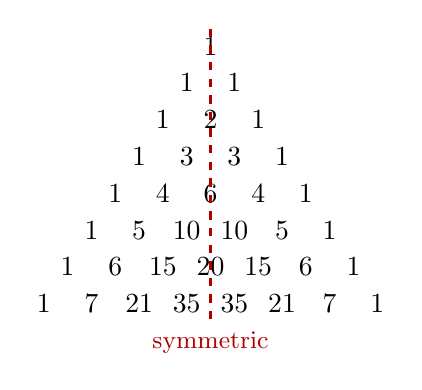
\begin{tikzpicture}[scale=0.55]

% Row 0
\node at (0, 0)          {1};
% Row 1
\node at (-0.55, -0.85)  {1};
\node at ( 0.55, -0.85)  {1};
% Row 2
\node at (-1.1,  -1.7)   {1};
\node at ( 0,    -1.7)   {2};
\node at ( 1.1,  -1.7)   {1};
% Row 3
\node at (-1.65, -2.55)  {1};
\node at (-0.55, -2.55)  {3};
\node at ( 0.55, -2.55)  {3};
\node at ( 1.65, -2.55)  {1};
% Row 4
\node at (-2.2,  -3.4)   {1};
\node at (-1.1,  -3.4)   {4};
\node at ( 0,    -3.4)   {6};
\node at ( 1.1,  -3.4)   {4};
\node at ( 2.2,  -3.4)   {1};
% Row 5
\node at (-2.75, -4.25)  {1};
\node at (-1.65, -4.25)  {5};
\node at (-0.55, -4.25)  {10};
\node at ( 0.55, -4.25)  {10};
\node at ( 1.65, -4.25)  {5};
\node at ( 2.75, -4.25)  {1};
% Row 6
\node at (-3.3,  -5.1)   {1};
\node at (-2.2,  -5.1)   {6};
\node at (-1.1,  -5.1)   {15};
\node at ( 0,    -5.1)   {20};
\node at ( 1.1,  -5.1)   {15};
\node at ( 2.2,  -5.1)   {6};
\node at ( 3.3,  -5.1)   {1};
% Row 7
\node at (-3.85, -5.95)  {1};
\node at (-2.75, -5.95)  {7};
\node at (-1.65, -5.95)  {21};
\node at (-0.55, -5.95)  {35};
\node at ( 0.55, -5.95)  {35};
\node at ( 1.65, -5.95)  {21};
\node at ( 2.75, -5.95)  {7};
\node at ( 3.85, -5.95)  {1};

\draw[kcpc-red, thick, dashed]
    (0, 0.4) -- (0, -6.35)
    node[below, kcpc-red] {\small symmetric};

\end{tikzpicture}

\vspace{0.3em}
{\small Note the symmetry: $\binom{n}{r} = \binom{n}{n-r}$}
\end{frame}

\begin{frame}{Worked Example}
        \includegraphics[width = 1.2 \linewidth]{PE53.png}
        
\end{frame}

\begin{frame}{Worked Example}
        Naive approach is to test each value separately, this gives $5050$ in total, and is slow to compute.

        \textbf{Take a step back and think}: have symmetry between $r$ and $n-r$, so only need to compute half the values.

        \textbf{Looking closer}: each value is the sum of previous terms.

        So can set up some 2D array in a DP-style, and if any term hits $1000000$, we know the sub-triangle below it is all above $100000$ too!
\end{frame}

\begin{frame}[fragile]{Worked Example}
    \textbf{Pseudocode}
        \begin{lstlisting}[language=Python]
COUNT = 0
C = [[0] * 101 for _ in range(101)]
for n in range(101):
    C[n][0] = 1
    for r in range(1, n // 2 + 1):
        C[n][r] = C[n-1][r-1] + C[n-1][r]
        if C[n][r] > 1000000:
            C[n][r] = float('inf')
            COUNT += 1
        C[n][n-r] = C[n][r]
print(COUNT)
    \end{lstlisting}
\end{frame}

\begin{frame}{A New Star}
    Very soon you'll run into problems like how many ways can 5 identical sweets be split into 3 bags?
    
    \vspace{1em}
    \centering
    \centering
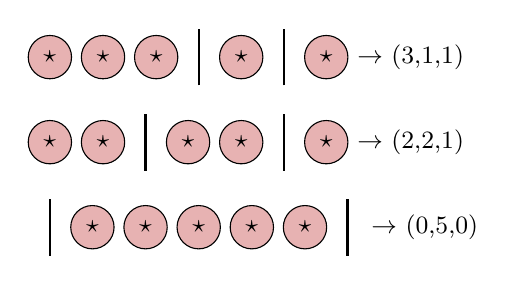
\begin{tikzpicture}[scale=0.9]

    % Row 1: 3,1,1
    \foreach \x in {0, 0.75, 1.5} {
        \node[draw, circle, fill=kcpc-red!30, minimum size=0.55cm, inner sep=0]
            at (\x, 0) {\small$\star$};
    }
    \draw[thick] (2.1, -0.4) -- (2.1, 0.4);
    \node[draw, circle, fill=kcpc-red!30, minimum size=0.55cm, inner sep=0]
        at (2.7, 0) {\small$\star$};
    \draw[thick] (3.3, -0.4) -- (3.3, 0.4);
    \node[draw, circle, fill=kcpc-red!30, minimum size=0.55cm, inner sep=0]
        at (3.9, 0) {\small$\star$};
    \node[right] at (4.2, 0) {\small $\to$ (3,1,1)};

    % Row 2: 2,2,1
    \foreach \x in {0, 0.75} {
        \node[draw, circle, fill=kcpc-red!30, minimum size=0.55cm, inner sep=0]
            at (\x, -1.2) {\small$\star$};
    }
    \draw[thick] (1.35, -1.6) -- (1.35, -0.8);
    \foreach \x in {1.95, 2.7} {
        \node[draw, circle, fill=kcpc-red!30, minimum size=0.55cm, inner sep=0]
            at (\x, -1.2) {\small$\star$};
    }
    \draw[thick] (3.3, -1.6) -- (3.3, -0.8);
    \node[draw, circle, fill=kcpc-red!30, minimum size=0.55cm, inner sep=0]
        at (3.9, -1.2) {\small$\star$};
    \node[right] at (4.2, -1.2) {\small $\to$ (2,2,1)};

    % Row 3: 0,5,0
    \draw[thick] (0, -2.8) -- (0, -2.0);
    \foreach \x in {0.6, 1.35, 2.1, 2.85, 3.6} {
        \node[draw, circle, fill=kcpc-red!30, minimum size=0.55cm, inner sep=0]
            at (\x, -2.4) {\small$\star$};
    }
    \draw[thick] (4.2, -2.8) -- (4.2, -2.0);
    \node[right] at (4.4, -2.4) {\small $\to$ (0,5,0)};

\end{tikzpicture}
\vspace{1em}
    
    \vspace{1em}
    Choosing which $2$ of $7$ positions are bars: $\dbinom{7}{2} = 21$
\end{frame}

\begin{frame}{Stars and Bars}
    \textbf{General Formula}

    Distributing $n$ identical items into $k$ distinct bins:
    $$\binom{n + k - 1}{k - 1}$$

    \vspace{0.5em}

    \textbf{Why?} We have $n$ stars and $k-1$ bars --- $n + k - 1$ symbols total.
    We choose which $k-1$ positions are bars.

    \vspace{0.5em}

    \textbf{Note:} this allows empty bins. If each bin must have $\geq 1$ item,
    give one to each bin first, then distribute $n - k$ items freely:
    $$\binom{n-1}{k-1}$$
\end{frame}



\section{Bijection and Proofs}
%MENTION SCHRODER-BERNSTEIN POTENTIALLY?
\begin{frame}{Dreamland}
    Wouldn't it be nice if instead of counting something we could count the elements of another set that just so happens to be the exact same size?

    That is the motivation behind \textbf{bijections:} one-to-one mappings.
\end{frame}

\begin{frame}{Definition}
Formally, a bijection between two sets $A, B$ is a function $f: A \rightarrow B$ such that:
\begin{itemize}
    \item \textbf{Injectivity} each element in $A$ maps to a different element in $B$, $f(a_i) = f(a_j) \Rightarrow a_i = a_j$
    \item \textbf{Surjectivity} each element in $B$ is mapped to by an element in $A$
\end{itemize}

\textbf{Key idea:} if $A, B$ are in bijection, $|A| = |B|$.

If we want to count $A$, but $B$ is a lot easier, we're happy $\smiley{}$
\end{frame}



\begin{frame}{Worked Example }
    \includegraphics[width = \linewidth]{pe15.png}
\end{frame}

\begin{frame}{Worked Example}
    Can accomplish this purely mathematically!

    Instead of counting paths (you will not get through them in a reasonable amount of time), call each move right an $R$ and each move down a $D$. Then \textbf{each path has an associated string!}

    Every string with $20$ R's and D's covers all valid paths.
\end{frame}

\begin{frame}{Worked Example}
    
    Try doing this with order, say you have $20$ R's in a row and try to insert D's: risk over-counting.

    \textbf{How do we do this properly?}

    Ignore ordering, consider every possible arrangement of the $40$ R's and D's, have $40!$ in total. Each R and each D are identical, so need to divide by a factor of $20!$, get $$\frac{40!}{20! *20!} = 137846528820$$
\end{frame}

\begin{frame}{Double-Counting}
    
   \textbf{A related technique:} count the same set two different ways to derive an identity.

    \textbf{Example:} Prove that $\binom{n}{0} + \binom{n}{1} + \dots + \binom{n}{n} = 2^n$
    
    \begin{itemize}
        \item \textbf{Left side:} sum over all possible subset sizes --- counts every subset of $\{1, \dots, n\}$ exactly once
        \item \textbf{Right side:} each element is either in or out, giving $2^n$ subsets total
        \item Same set, counted two ways $\implies$ they must be equal \qed
    \end{itemize}
\end{frame}

\begin{frame}{Double-Counting Example}
    \textbf{Claim}: $n$ points on a circle, every pair connected, no three chords concurrent inside. The number of interior intersections is $\binom{n}{4}$
\end{frame}
% ------------------------------------------------

\section{Inclusion-Exclusion}
%WILL STEAL DIAGRAMS FROM THIS FROM OTHER SOURCES UNLESS MARCELL REALLY GOOD WITH TIKZ
\begin{frame}{Why Bother}
    \textbf{Motivation:} If I need to count the number of events in A and B, what do I need to do to ensure that I haven't double counted anything?

    What about for 3 sets? Or more?
    \vspace{0.5em}
\end{frame}

\begin{frame}{Venn Diagrams}
\centering
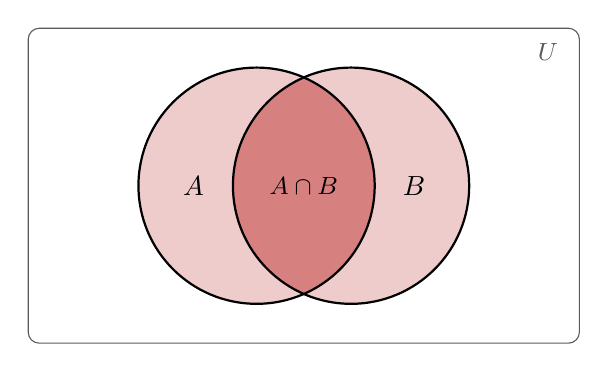
\begin{tikzpicture}
    \draw[rounded corners, kcpc-muted] (-3.5,-2) rectangle (3.5,2);
    \node[kcpc-muted] at (3.1,1.7) {\small$U$};

    \begin{scope}
        \clip (-0.6,0) circle (1.5);
        \fill[kcpc-red!20] (-0.6,0) circle (1.5);
    \end{scope}
    \begin{scope}
        \clip (0.6,0) circle (1.5);
        \fill[kcpc-red!20] (0.6,0) circle (1.5);
    \end{scope}
    \begin{scope}
        \clip (-0.6,0) circle (1.5);
        \clip (0.6,0) circle (1.5);
        \fill[kcpc-red!50] (-0.6,0) circle (1.5);
    \end{scope}

    \draw[thick] (-0.6,0) circle (1.5);
    \draw[thick] (0.6,0) circle (1.5);

    \node at (-1.4,0) {$A$};
    \node at (1.4,0) {$B$};
    \node at (0,0) {\small$A\cap B$};
\end{tikzpicture}

\vspace{0.5em}
When we add $|A| + |B|$, we count $A \cap B$ \textbf{twice}. So:
$$|A \cup B| = |A| + |B| - |A \cap B|$$
\end{frame}

\begin{frame}{3-Circle Diagram}
    \centering
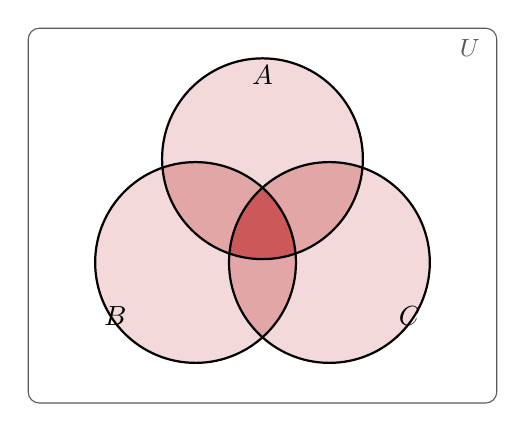
\begin{tikzpicture}[scale=0.85]
    \draw[rounded corners, kcpc-muted] (-3.5,-2.8) rectangle (3.5,2.8);
    \node[kcpc-muted] at (3.1,2.5) {\small$U$};

    \fill[kcpc-red!15] (0,0.85) circle (1.5);
    \fill[kcpc-red!15] (-1.0,-0.7) circle (1.5);
    \fill[kcpc-red!15] (1.0,-0.7) circle (1.5);

    \begin{scope}
        \clip (0,0.85) circle (1.5);
        \clip (-1.0,-0.7) circle (1.5);
        \fill[kcpc-red!35] (0,0.85) circle (1.5);
    \end{scope}
    \begin{scope}
        \clip (0,0.85) circle (1.5);
        \clip (1.0,-0.7) circle (1.5);
        \fill[kcpc-red!35] (0,0.85) circle (1.5);
    \end{scope}
    \begin{scope}
        \clip (-1.0,-0.7) circle (1.5);
        \clip (1.0,-0.7) circle (1.5);
        \fill[kcpc-red!35] (-1.0,-0.7) circle (1.5);
    \end{scope}
    \begin{scope}
        \clip (0,0.85) circle (1.5);
        \clip (-1.0,-0.7) circle (1.5);
        \clip (1.0,-0.7) circle (1.5);
        \fill[kcpc-red!65] (0,0.85) circle (1.5);
    \end{scope}

    \draw[thick] (0,0.85) circle (1.5);
    \draw[thick] (-1.0,-0.7) circle (1.5);
    \draw[thick] (1.0,-0.7) circle (1.5);

    \node at (0,2.1) {$A$};
    \node at (-2.2,-1.5) {$B$};
    \node at (2.2,-1.5) {$C$};
\end{tikzpicture}
\end{frame}

\begin{frame}{Three Sets}
    Adding $|A|+|B|+|C|$ overcounts pairwise intersections and 
    undercounts the triple intersection. Fixing this gives:

    \vspace{0.5em}

    {\small
    $$|A \cup B \cup C| = |A|+|B|+|C| - |A\cap B| - |A\cap C| - |B\cap C| + |A\cap B\cap C|$$
    }

    \vspace{0.5em}

    \textbf{General pattern:} add individuals, subtract pairs, add triples, subtract quadruples $\dots$

    $$\left|\bigcup_{i=1}^n A_i\right| = \sum_i|A_i| - \sum_{i<j}|A_i\cap A_j| + \sum_{i<j<k}|A_i\cap A_j\cap A_k| - \cdots$$
\end{frame}


\begin{frame}{Derangements}
    \textbf{Application:} How many permutations of $\{1, \dots, n\}$ have \textbf{no fixed points}?

    \vspace{0.5em}

    Let $A_i$ = permutations where element $i$ is in position $i$. We want $\left|\overline{A_1} \cap \cdots \cap \overline{A_n}\right|$.

    By PIE:
    $$D_n = n!\sum_{k=0}^{n} \frac{(-1)^k}{k!}$$

    \vspace{0.3em}

    \begin{itemize}
        \item $D_1 = 0, \quad D_2 = 1, \quad D_3 = 2, \quad D_4 = 9$
        \item As $n \to \infty$, $D_n / n! \to e^{-1} \approx 0.368$
    \end{itemize}

    \vspace{0.3em}

    \textbf{Intuition:} roughly $1/e$ of all permutations are derangements regardless of $n$.
\end{frame}
% ------------------------------------------------

\section{Extension}
%LIKELY TO MENTION 

\begin{frame}{Further Directions}
     \textbf{Catalan Numbers}
    \begin{itemize}
        \item $C_n = \dfrac{1}{n+1}\dbinom{2n}{n}$ counts many things like bracket sequences and non-crossing grid paths
        \item $C_0=1, C_1=1, C_2=2, C_3=5, C_4=14$
    \end{itemize}

    \vspace{0.5em}

    \textbf{Burnside's Lemma}
    \begin{itemize}
        \item Counts distinct objects under symmetry --- e.g.\ necklaces, colourings
        \item Requires group theory (see Groups notes in reading list)
        \item Answer to the necklace problem from the start of the session!
    \end{itemize}

    \vspace{0.5em}

    Full treatment in the supplementary reading document.
    
\end{frame}

% ------------------------------------------------

\section{Problem Sheet}
\begin{frame}
    Check it out online!

    \begin{itemize}
        \item Problems available on the KCPC Discord and website
        \pause
        \item Work individually or in small groups
        \pause
        \item Covers: counting, combinations, bijections, inclusion-exclusion
        \pause
        \item We will review selected solutions afterwards
    \end{itemize}
\end{frame}
% ------------------------------------------------

\section{Final Remarks}
\begin{frame}
    This may be annoying at first but do keep trying!

    \begin{itemize}
        \item Multiplication principle --- independent stages multiply
        \item Factorials and binomial coefficients --- ordered vs unordered
        \item Stars and bars --- distributing identical items
        \item Bijections --- count something easier instead
        \item Inclusion-exclusion --- correct for overcounting
    \end{itemize}

    \vspace{0.5em}

    These will come up constantly. The only way to get faster at spotting them is to \textbf{do problems}.
\end{frame}
% ------------------------------------------------

\begin{frame}{Further Reading}

    \begin{itemize}
    
        \item A document containing relevant supplementary + research reading will be available on the KCPC website (for this workshop) and the KCPC Discord Resource section for you to check out :D
    
    \end{itemize}
    
\end{frame}

% ------------------------------------------------

\end{document}